Pe lângă facilitățile de extensibilitate oferite de utilizarea serviciilor cloud din cadrul "Amazon Web Services", arhitectura aplicației "Surf" prezintă următoarele puncte de extensie:

\begin{itemize}
	\item{Adăugare rapidă și ușoară de noi servicii cloud în cluster-ul aplicației, datorită structurii decuplate și configurabile a mecanismului de generare a infrastructurii;}
	\item{Asigurarea infrastructurii crawler-ului în mai multe regiuni globale, în conformitate cu politicile de globalizare AWS, astfel încât aplicația "Surf" să poată fi folosită la scară largă;}
	\item{Posibilitatea de a adăuga funcții Lambda de tip plug-in, alături de mecanismului de parcurgere și procesare a informațiilor din cadrul paginilor web vizitate de către crawler (\textit{"Figura 11"}).}
\end{itemize}

\begin{figure}[ht]
\begin{center}
	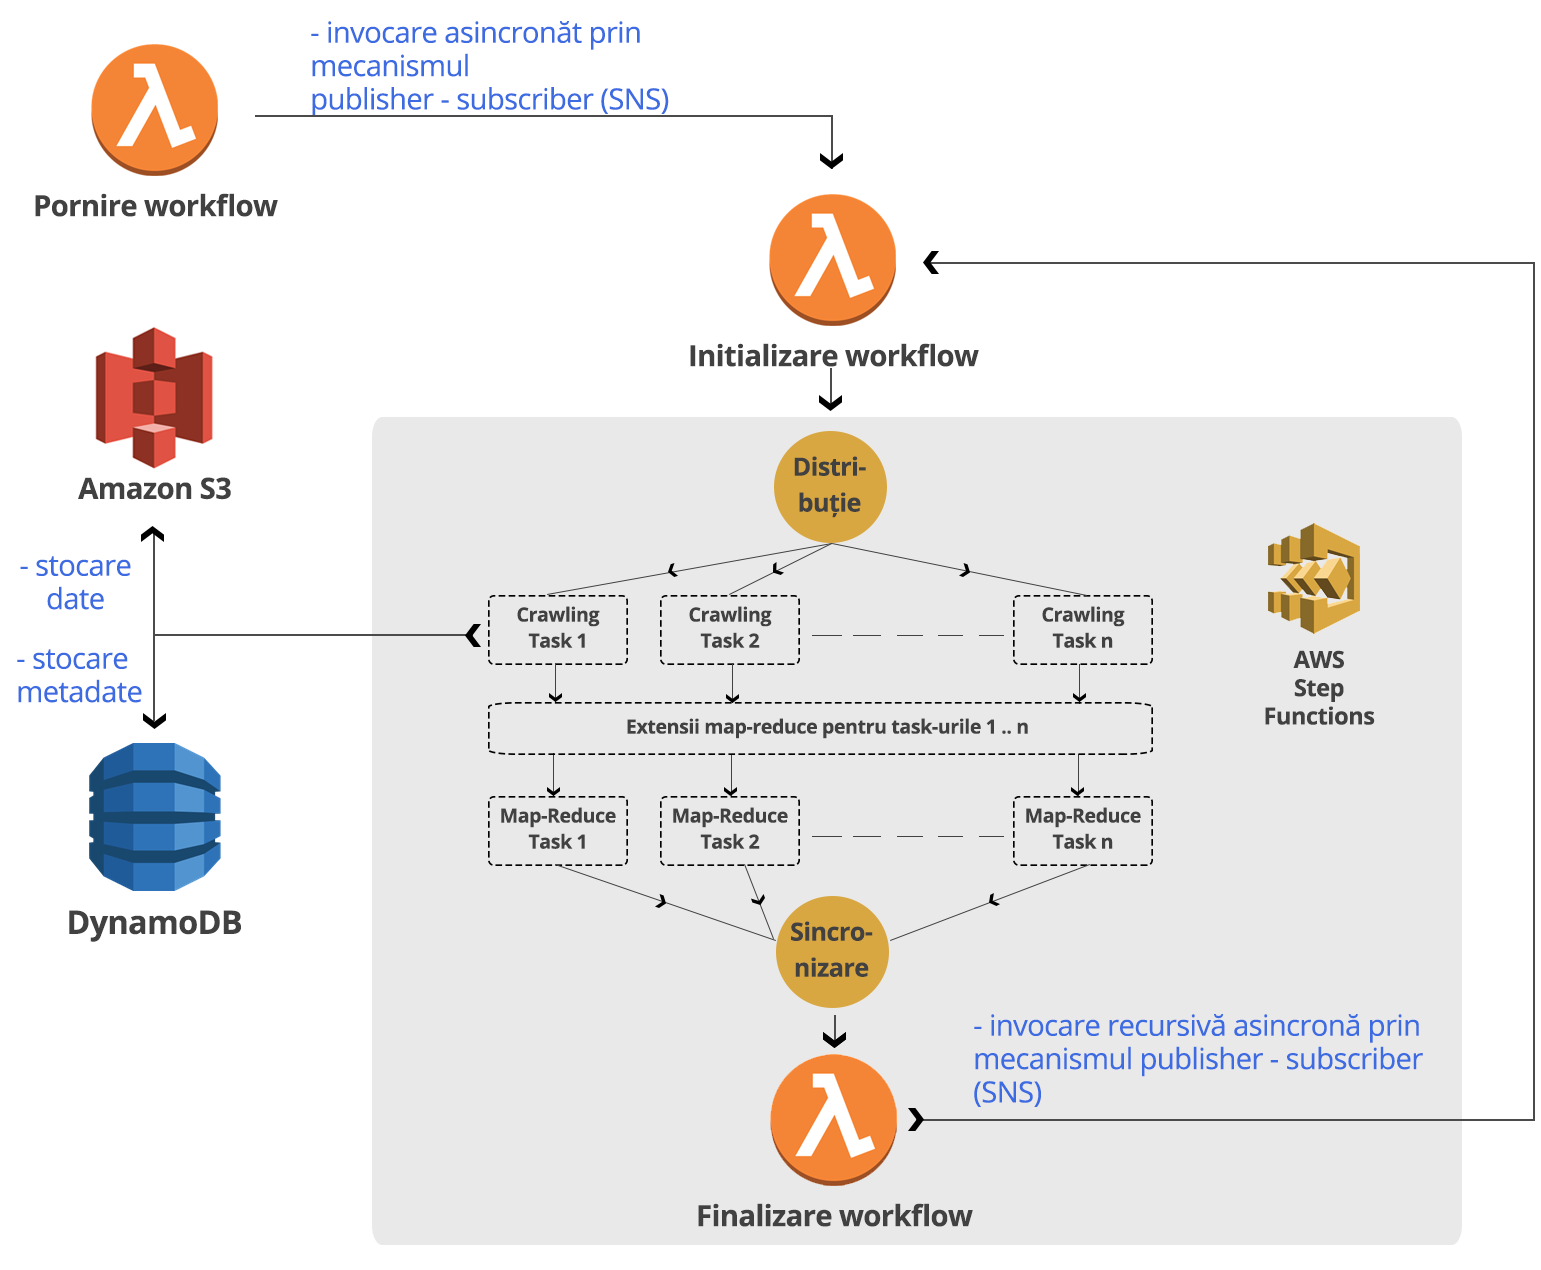
\includegraphics[keepaspectratio, width=0.9\textwidth]{proces-crawling-cu-pluginuri.png}
	\caption{Plugin-uri adăugate procesului de crawling \cite{diagram-icons-sources, aws-icons-source}}\par\medskip 

\end{center}
\end{figure}